    %!xelatex = 'xelatex --halt-on-error %O %S'

\documentclass{thuemp}
\begin{document}

% 标题,作者
\emptitle{微波电子自旋共振与铁磁共振实验研究}
\empauthor{王驰}{王合英}

% 奇数页页眉
\fancyhead[CO]{{\footnotesize 王驰: 微波电子自旋共振与铁磁共振实验研究}}

%%%%%%%%%%%%%%%%%%%%%%%%%%%%%%%%%%%%%%%%%%%%%%%%%%%%%%%%%%%%%%%%
% 关键词 摘要 首页脚注
%%%%%%%%关键词
\Keyword{电子自旋共振,铁磁共振,微波技术,扫场,朗德$g$因子}
\twocolumn[
\begin{@twocolumnfalse}
\maketitle

%%%%%%%%摘要
\begin{empAbstract}
    本实验利用微波共振技术研究了电子自旋共振(ESR)和铁磁共振(FMR)现象。通过搭建微波系统,分别对DPPH自由基样品和多晶铁氧体在交变磁场中的功率吸收特性进行研究。在DPPH自由基样品中,测得电子$g$因子为$2.049 \pm 0.005$,与公认值$g_e=2.0023$接近;在多晶铁氧体样品中,测得铁磁共振$g$因子为$2.016 \pm 0.008$,线宽$\Delta B = \SI{1.7}{\milli\tesla}$,弛豫时间$\tau \approx \SI{262}{\nano\second}$。实验验证了磁共振条件$h\nu = g\mu_B B$,并比较了洛伦兹线型、高斯线型及水晶球函数对铁磁共振峰的拟合效果。实验结果为研究顺磁以及铁磁性材料对交变电磁场的响应提供了重要参照。
\end{empAbstract}

%%%%%%%%英文标题、作者、摘要、关键词
\emptitleEn{Electron Spin Resonance and Ferromagnetic Resonance Experiments}
\empauthorEn{Chi Wang}{Heying Wang}
\KeywordEn{Electron spin resonance, Ferromagnetic resonance, Microwave technology, Sweep field, Landé g-factor}

\begin{empAbstractEn}
    This experiment investigates the phenomena of electron spin resonance (ESR) and ferromagnetic resonance (FMR) using microwave resonance technology. By constructing a microwave system, the power absorption characteristics of these samples in an alternating magnetic field are studied. In the DPPH radical sample, the measured electron g-factor is $2.049 \pm 0.005$, close to the accepted value of $g_e=2.0023$; in the multicrystalline ferrite sample, the measured ferromagnetic resonance g-factor is $2.016 \pm 0.008$, with a linewidth of $\Delta B = \SI{1.7}{\milli\tesla}$ and a relaxation time of $\tau \approx \SI{262}{\nano\second}$. The experiment verifies the magnetic resonance condition $h\nu = g\mu_B B$ and compares the fitting effects of Lorentzian, Gaussian, and Crystall Ball functions on the ferromagnetic resonance peak. The experimental results provide important references for studying the response of paramagnetic and ferromagnetic materials to alternating electromagnetic fields.
\end{empAbstractEn}

%%%%%%%%首页角注
\empfirstfoot{2025-04-20}{2025-05-07}{2022012259}{chi-wang22@mails.tsinghua.edu.cn}
\end{@twocolumnfalse}
]
%%%%%%%%!首页角注可能与正文重叠,请通过调整正文中第一页的\enlargethispage{-3.3cm}位置手动校准正文底部位置:
%%%%%%%%%%%%%%%%%%%%%%%%%%%%%%%%%%%%%%%%%%%%%%%%%%%%%%%%%%%%%%%%
%  正文由此开始
\wuhao 
%  分栏开始

\section{引言}
\enlargethispage{-3.3cm}
\section{实验内容}

\subsection{电子自旋共振}

\subsubsection{电子自旋共振的描述}

当具有未成对电子的物质置于外加磁场中时,电子自旋会与磁场相互作用,导致能级分裂。能级分裂宽度$\Delta E$与外加磁场强度$B$以及电子磁矩$\mu$有关,满足关系式:

\begin{equation}
\Delta E = \mu B
\end{equation}

其中电子磁矩可以进一步用Bohr磁子$\mu_B = \frac{e\hbar}{2m_e}$和朗德$g$因子表示为:

\begin{equation}
\mu = g \mu_B
\end{equation}

在交变磁场作用下,当电磁波频率$\nu$与能级分裂频率相等时,电子自旋会发生共振跃迁,对电磁波的吸收达到极大,满足关系式:

\begin{equation}
h \nu  = \Delta E = g \mu_B B
\end{equation}

在电子由低能态跃迁至高能态后,通过与晶格以及周围电子的相互作用,系统回到低能态,伴随各向电磁波辐射,此过程称为弛豫。由于弛豫作用的存在,即使是在共振条件完全满足时,稳态下仍然会有一定数量的电子处于低能态,因此能在实验上测量到一稳定的共振吸收。

\subsubsection{测量系统与样品选择}

对于电子自旋共振,朗德$g$因子值接近于2;实验室中电磁铁一般可产生$0.1 ~\text{T} $至$1.0~\text{T}$的磁场,对应于共振频率在数个\si{\giga\hertz},因而为测量电子自旋共振信号,需要使用微波波段电磁波源,以及波导、谐振腔等微波器件。

在本次实验中,我们使用北京大华DH1121A型3\si{\centi\meter}固态信号源作为微波源,配合BJ-100型波导管等微波器件,以及岩崎(IWATSU)SS-7802A型模拟示波器,对电子自旋共振和铁磁共振现象进行研究。如图【】所示,样品置于谐振腔内,通过一电磁铁提供磁场;微波源输出的微波信号通过隔离期、衰减器、环行器传输至反射式谐振腔,并在与样品相互作用后,再通过环行器以及波导管传输至晶体检波器,最终形成可读出的线信号。

由于产生微波的元件本身频率调节有一定难度,在实验上通过常通过调节外加磁场,并观察微波功率吸收随之发生的变化,以吸收最大时对应的磁感应强度与微波源频率计算出朗德$g$因子。

在常见化合物中,电子通常以自旋相反的电子对存在,难以产生自旋共振信号。历史上曾使用X射线照射小分子有机物,引起部分分子电离,进而得到含孤电子体系用于测量。在本次实验中,我们使用1,1-二苯基-2-(1,4,6-三硝基苯基)肼自由基(1,1-Diphenyl-2-picrylhydrazyl radical, DPPH)作为实验材料:DPPH本身是一种相对稳定的自由基,其分子中含有一个未成对电子(如\ref{fig:DPPH}),能够产生较强的自旋共振信号。\

\begin{figure}[H]
    \centering
    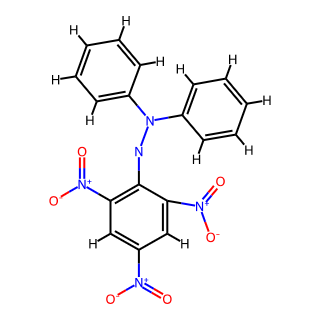
\includegraphics[width=0.5\linewidth]{./DPPH_molecule.png}
    \caption{DPPH分子结构示意图} \label{fig:DPPH}
\end{figure}

在本部分测量中,DPPH样品被置于反射式谐振腔内,其几何尺寸可调,以适应于不同频率的微波信号。

在实验之初,需要选定适当微波源频率,并由此计算波导内波长$\lambda_g$,进而调整反射式谐振腔腔长,以及被测量样品的摆放位置。

所使用波导管为BJ-100型矩形波导,其宽度$a=22.86\pm0.07$ \si{\milli\meter},对应主模频率区间为$8.20 \approx 12.50$ \si{\giga\hertz}。

综合微波源以及波导管特性,选取微波源输出频率在$9~\text{GHz}$附近,设定输出后借助直读式频率计读出$\nu  = 8.960 \pm 0.005$ \si{\giga\hertz},对应计算得到波长$\lambda$以及波导波长$\lambda_g$:

\begin{equation}
\lambda = \frac{c}{\nu} = 33.46 ~\text{mm}
\end{equation}

\begin{equation}
\lambda_g = \frac{\lambda}{\sqrt{1 - \left(\frac{\lambda}{2a}\right)^2}} = 49.10 ~\text{mm}
\end{equation}

在反射式谐振腔中,为使样品的自旋共振信号最大,应当使谐振腔内电磁场形成驻波,且样品应放置在腔内驻波磁感应强度幅值最大处。谐振腔长$L$,样品与谐振腔端面距离$d$和波导波长$\lambda_g$满足以下关系:

\begin{equation}
L = \frac{n}{2}\lambda_g \quad (n \in \mathbb{Z}^+)
\end{equation}

\begin{equation}
d = \frac{m}{2}\lambda_g \quad (m \in \mathbb{Z}^+)
\end{equation}

在本次实验中,选取谐振腔长$L=3\lambda_g\approx$,样品与谐振腔端面距离$d=\frac{3}{2}\lambda_g\approx$。为确认取到谐振腔内驻波磁感应强度幅值最大处,通过反复联合调节样品位置和谐振腔长度,观察,最终得到谐振腔内驻波磁感应强度幅值最大处的样品位置$d \approx 73.4 $\si{\milli\meter}。

\subsubsection{借助扫场信号观察电子自旋共振信号}

电子自旋共振频宽可能较窄,且晶体检波器-微安表系统对微波功率变化的响应较慢,因此在实验中借助磁共振实验仪的扫场功能,使用示波器确认共振发生所对应的中心频率:在一恒定励磁电流基础上,加一周期变化且幅值较小的周期信号,即“扫场信号”,由此样品电子自旋对磁感应强度变化的响应,会在时域上被展开成一个脉冲信号,显示在示波器上;调节励磁电流中心值$B$,直至这一脉冲信号中心落在示波器屏幕中心位置,此时$B_0$即满足样品电子自旋共振条件。

在本实验中,扫场信号为一锯齿波,因而在一个扫描周期内,会在示波器上将显示两个脉冲信号:第一个脉冲信号对应于扫场信号上升段,第二个脉冲信号对应于扫场信号下降段。判定样品电子自旋共振条件时,实际取两脉冲信号中心值近似相等作为判据。

\subsection{铁磁共振}

\subsubsection{铁磁共振的描述}

在铁磁体中,电子自旋方向之间存在显著关联,在外加适当频率交变磁场时,会相类似地表现出自旋共振现象,整体宏观磁化矢量发生进动,并伴有对对应频率电磁波能量的强烈吸收。

在铁磁体系中,弛豫现象较之于电子自旋共振更为显著。为描述顺磁系统的宏观磁矩进动以及弛豫现象,通常使用Bloch方程描述宏观磁化矢量$\symbf{M}$的时间演化:

\begin{equation}
\begin{aligned}
    \frac{\mathrm{d} M_x}{\mathrm{d} t} &= \gamma (\symbf{M} \times \symbf{B'})_x - \frac{M_x}{\tau_2} \\
    \frac{\mathrm{d} M_y}{\mathrm{d} t} &= \gamma (\symbf{M} \times \symbf{B'})_y - \frac{M_y}{\tau_2} \\
    \frac{\mathrm{d} M_z}{\mathrm{d} t} &= \gamma (\symbf{M} \times \symbf{B'})_z - \frac{M_z - M_z^0}{\tau_1}
\end{aligned}
\end{equation}

其中已选取坐标轴使得外加磁场$\mathbf{B}$沿$z$轴方向,$\symbf{B'}$为外加的交变磁场,$\tau_1$和$\tau_2$分别为纵向弛豫时间和横向弛豫时间,分别对应自旋-晶格相互作用和自旋-自旋相互作用。

类似于电子自旋共振,铁磁共振也会在外加磁感应强度满足特定条件时发生共振跃迁,伴随对对应频率电磁波能量的强烈吸收。对于铁磁物质,这一吸收作用还可以通过交变磁场下整体复磁导率$\tilde\mu $来描述:

\begin{equation}
    \tilde\mu = \mu' + i\mu''
\end{equation}

其中$\mu'$对应于其在稳定磁场下的磁导率,$\mu''$对应于交变磁能在铁磁体中耗散的部分。调整外加磁感应强度至发生铁磁共振时,$\omega = \frac{g}{\mu_B\hbar} B_0$,$\mu''$也会达到极大值,且存在一共振展宽$\Delta B$对应于铁磁共振的频宽。在本实验中,我们定义$\mu'' = \frac 1 2 \mu''_{\mathrm{max}}$时对应的磁感应强度间隔$(B_1 - B_2)$作为$\Delta B$。

在一般情况下,$\tau_1 = \tau_2 \approx 2/\gamma \Delta B$;方便起见将$\tau_1, \tau_2$统称为弛豫时间$\tau$,则有:

\begin{equation}
    \tau = \frac{2}{\gamma\Delta B} = \frac{4\pi}{\nu}\frac{B_0}{\Delta B}
\end{equation}



\subsubsection{测量系统与样品选择}

在铁磁共振实验中,我们将使用传输式谐振腔,对多晶铁氧体样品的铁磁共振进行测量。如图【】,微波源产生的微波信号经过隔离器、衰减器等微波器件进入传输式谐振腔,并在与样品作用后进入下一段波导,进而通过其中的晶体检波器以及与之相连的检流计,读出透射微波功率。在本次测量中,我们将假定检波二极管工作在信号电流与场强平方成正比的区间,此时读出的电流即正比于功率。

\section{实验结果与分析}

\subsection{电子自旋共振朗德$g$因子计算}

调节励磁电流中心值以及扫场幅度,观察到励磁电流为$I_{m,0} = 1.821$\si\ampere 时,示波器上显示的两个脉冲信号中心位置相近,且幅值均较大。结合实验所使用电磁体特性:

\begin{equation}
    B = 0.0152 ~\text{\si\tesla} + 0.1632 ~\text{\si\tesla / \si\ampere} \cdot I_m
\end{equation}

得到此时样品电子自旋共振条件下的磁感应强度为$B_0 = 0.3123$ \si\tesla。给出$g$因子测量值:

\begin{equation}
g = \frac{h \nu}{\mu_B B_0} = \frac{4\pi m_e}{e} \frac{\nu}{B_0}\approx 2.049
\end{equation}

测量结果与公认的电子$g$因子已经相当接近。

\subsection{铁磁共振朗德$g$因子计算}

在此部分实验中,设定频率为$\nu = 9.029 \pm 0.005~\text{\si{\giga \hertz}}$为确定透射功率取最小值,以及透射功率恰好取到$P_{1/2}$时的外加磁场,对测量得到的功率-磁场关系,通过使用适当函数进行拟合,确定吸收峰中心值,并反解得到$B_1, B_2$,进而利用【】式计算得到$\Delta B$。

选用Lorentz线型作为信号形状进行拟合,结果如下:

\begin{figure}[H]
    \centering
    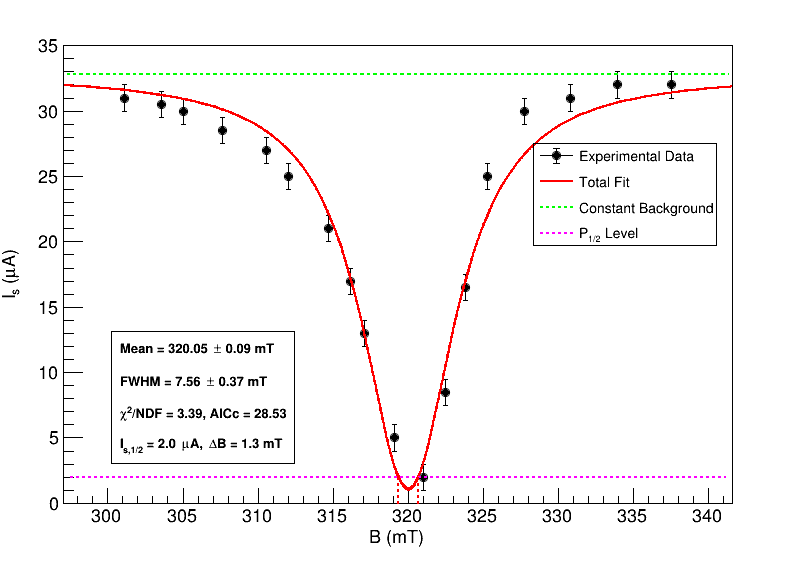
\includegraphics[width=0.9\linewidth]{../Data/FMR_ConstantBg_LorentzPeak.png}
    \caption{铁磁共振透射功率与外加磁场关系图} \label{fig:gmr_gradient}
\end{figure}

拟合得到参数如下:

\begin{table}[H]
    \centering
    \captionnamefont{\wuhao\bf\heiti}
    \captiontitlefont{\wuhao\bf\heiti}
    \caption{铁磁共振信号拟合结果} \label{tab:FMR_fit}
    \liuhao
    \begin{tabular}{cccc}
        \toprule
        中心值 & 半高全宽(FWHM) & 信号幅度 & 背景信号高度 \\
        $B_0/\text{\si\tesla}$ & $\Gamma_B/\text{\si\tesla}$ & $A/\text{\si{\micro\ampere}}$ & $I_{S,0}$\\
        \midrule
        0.32 & 7.5 & 31.8 & 32.8 \\
        \bottomrule
    \end{tabular}
\end{table}

此时可以根据共振峰中心值$B_0$求出$g$因子:

\begin{equation}
g = \frac{h \nu}{\mu_B B_0} = \frac{4\pi m_e}{e} \frac{\nu}{B_0}\approx 2.016
\end{equation}

如此得到的结果与自由电子$g$因子接近。

\subsection{铁磁共振弛豫时间分析}

根据表格\ref{tab:FMR_fit}进一步求出与$P_r, P_0, P_{1/2}$分别对应的信号电流值$I_r, I_0, I_{1/2}$,反解得到$B_{1}, B_{2}$:

\begin{table}[H]
    \centering
    \captionnamefont{\wuhao\bf\heiti}
    \captiontitlefont{\wuhao\bf\heiti}
    \caption{铁磁共振弛豫时间分析结果表} \label{tab:FMR_relax}
    \liuhao
    \begin{tabular}{cccccc}
        \toprule
        无吸收时 & 共振情形 & $\mu''$半宽 &
            \multicolumn{2}{c}{$\mu''$半宽所对应}\\
        信号电流 & 信号电流 & 信号电流     &  
            \multicolumn{2}{c}{外加磁场}\\
        $I_{0}/\text{\si{\micro\ampere}}$ & 
            $I_{r}/\text{\si{\micro\ampere}}$ &
            $I_{1/2}/\text{\si{\micro\ampere}}$&
            $B_1/\text{\si{\milli\tesla}}$ &
            $B_2/\text{\si{\milli\tesla}}$ \\ 
        \midrule
        32.80& 1.02 & 1.98 & 319.4 & 320.7 \\
        \bottomrule
    \end{tabular}
\end{table}

其中,根据检波二极管特性$I \propto E^2 \propto P$,使用以下关系式:

\begin{equation}
    I_{1/2} = \frac{2P_0P_r}{P_0+P_r}
\end{equation}

由以上结果,计算得:
\begin{equation}
    \Delta B = |B_1 - B_2| = 1.7 ~\text{\si{\milli\tesla}}
\end{equation}

\begin{equation}
    \tau = \frac{2}{\gamma\Delta B}
         = \frac{4\pi}{\nu}\frac{B_0}{\Delta B}
         \approx 262 ~ \text{ns}
\end{equation}

值得注意的是,$P_{1/2}$已经极接近$P_r$,且此区间内对共振峰的拟合有较大不确定性,因而$\Delta B$以及由此导出的$\tau$本身也有较大不确定度。对$\tau$若要进行更精确的测量,需要在靠近共振峰处取更多数据点。

\section{结论}

本实验通过微波电子自旋共振和铁磁共振现象的研究,成功测量了DPPH自由基样品的电子$g$因子为$2.049 \pm 0.005$,与自由电子的公认值$g_e=2.0023$接近而仍有一定偏差,提示其为顺磁中心而同时受到了分子内其他电子的作用,展示了微波电磁自旋共振方法在化学中物质结构分析领域的重要价值;对多晶铁氧体样品测得铁磁共振$g$因子为$2.016 \pm 0.008$,线宽$\Delta B = \SI{1.7}{\milli\tesla}$,弛豫时间$\tau \approx \SI{262}{\nano\second}$。实验验证了磁共振条件$h\nu = g\mu_B B$,并比较了洛伦兹线型、高斯线型及水晶球函数对铁磁共振峰的拟合效果,确认了洛伦兹线型对铁磁共振的描述最为适宜,且符合其阻尼共振的物理机制。实验结果为研究顺磁以及铁磁性材料对交变电磁场的响应提供了重要参照。



%%%%%%%%%%%%%%%%%%%%%%%%%%%%%%%%%%%%%%%%%%%%%%%%%%%%%%%%%%%%%%%%
%  参考文献
%%%%%%%%%%%%%%%%%%%%%%%%%%%%%%%%%%%%%%%%%%%%%%%%%%%%%%%%%%%%%%%%
\renewcommand\refname{\heiti\wuhao\centerline{参考文献}\global\def\refname{参考文献}}
\vskip 12pt

\let\OLDthebibliography\thebibliography
\renewcommand\thebibliography[1]{
  \OLDthebibliography{#1}
  \setlength{\parskip}{0pt}
  \setlength{\itemsep}{0pt plus 0.3ex}
}

{
\renewcommand{\baselinestretch}{0.9}
\liuhao
\bibliographystyle{gbt7714-numerical}
\bibliography{./Report/TempExample}
}
\newpage
\appendix

\section{关于未测量电子自旋共振信号与样品位置关联的说明}

在部分实验过程中,实验人员尝试通过螺杆调节样品位置,以研究样品位置对电子自旋共振信号的影响。在实验开始阶段,实验人员注意到调节螺杆出现卡阻现象,尝试通过加大调节力度进行克服,随后阻尼感消失,但在测量中发现样品位置与电子自旋共振信号之间关联并不显著。在撤开电磁铁并准备调整微波系统连接方式时,实验人员发现反射式谐振腔的样品位置螺杆与谐振腔连接螺丝之间的塑料连接件已经断裂脱落,推断为在调节样品位置时,螺杆与谐振腔连接螺丝之间的塑料连接件与电磁铁磁极卡阻,进而在后续调节中断裂脱落。由于当时实验室内并无备件,经实验指导教师许可放弃本部分测量。

\section{铁磁共振信号拟合函数的选择}

对铁磁共振信号,在拟合过程中曾先后使用高斯型、洛伦兹型和水晶球函数作为信号函数。其中,水晶球函数表达式为:


以上各组合拟合结果如下:


其中,水晶球函数虽然拟合描述最好,但是总共使用6个拟合参数,数量过多,存在潜在的过拟合风险。结合曲线符合程度,选择使用洛伦兹型峰描述共振信号。



\section{源代码获取}

本实验所使用的代码,包括本篇报告的\LaTeX 源码,均可从\url{github.com/Eric100911/mpl-ESR-FMR}下载。

\end{document}